\documentclass[output=paper]{langsci/langscibook} 
\ChapterDOI{10.5281/zenodo.5040316}
\author{Yijun Duan\affiliation{National Institute of Advanced Industrial Science and Technology} and Adam Jatowt\affiliation{University of Innsbruck}
and  Masatoshi Yoshikawa\affiliation{Kyoto University}}
\title[Document collection representation by diachronic linguistic periodization]
      {Structured representation of temporal document collections by diachronic linguistic periodization}
 
\abstract{Language is our main communication tool. Deep understanding of its evolution is imperative for many related research areas including history, humanities, social sciences, etc. as well as for effective temporal information retrieval. 
To this end, we are interested in the task of segmenting long-term document corpora into naturally coherent periods based on the embodied evolving word semantics. There are many benefits of such segmentation including better representation of content in long-term document collections and support for modeling and understanding semantic drift. We propose a two-step framework for learning time-aware word semantics and periodizing document archive. The effectiveness of our model is demonstrated on the New York Times corpus spanning from 1990 to 2016.}

\begin{document}
\maketitle


\section{Introduction}

Language is an evolving and dynamic construct. Awareness of the necessity and possibilities of large scale analysis of the temporal dynamics on linguistic phenomena has increased considerably in the last decade \citep{zhang-etal-2015-omnia, yao2018dynamic, chapters/01}.
Temporal dynamics play an important role in many time-aware information retrieval (IR) tasks. For example, when retrieving documents based on their embeddings, one needs accurate representations of content by temporal embedding vectors. 

It is intuitive that if an IR system is required to effectively return information from a target time period $T_a$, it may fail to do so if it is unable to capture the change in context between $T_a$ and the current time, or just another time period in the past $T_b$. To which extent is the context of $T_a$ different from that of $T_b$? Are there any turning points in the interval between $T_a$ and $T_b$ when a significant context change occurred, or do $T_a$ and $T_b$ belong to the same stage in the evolving process of language rather? The capability of answering such questions is crucial for effective IR systems when coping with time-aware tasks. However, to the best of our knowledge, the research problem of distinguishing key stages in the evolution's trajectory of language still remains a challenge in the field of temporal IR.

\begin{sloppypar}
Traditionally, a language's diachrony is segmented into pre-determined periods (e.g., the ``Old", ``Middle" and ``Modern" eras for English) \citep{schatzle2019diahclust}, which is problematic, since such an approach may yield results concealing the true trajectory of a phenomenon (e.g., false assumption on abrupt turning point about the data). Moreover, these traditional segments are very coarse and can be easily obscured and derived from arbitrary and non-linguistic features \citep{degaetano2018using}. 
Thanks to accumulated large amounts of digitized documents from the past, it is now possible to employ large scale data-driven analyses for uncovering patterns of language change. Thus, instead of blindly adopting a pre-determined periodization scheme, data-driven approaches, which reflect actual changes in the data, and which are able to achieve meaningful generalizations, can be applied. This can not only help with evolutionary linguistic studies by providing data-driven evidence, but could also support better understanding of variations in performance of diverse temporal IR systems on different periods of a temporal document collection. Furthermore, automatic periodization can be also beneficial for many less-researched languages for which there may not be a sufficient number of historical linguistics-oriented studies and findings.
\end{sloppypar}

In this study, we design a data-driven approach for segmenting a temporal document collection (e.g., a long-term news article archive) into natural, linguistically coherent periods, thanks to which we can both capture the features involved in diachronic linguistic change, as well as identify the time periods when the changes occurred. Our approach is generic and can be applied to any diachronic data set. The detected periods could then be applied in diverse temporal IR scenarios, such as temporal analog retrieval and archival document recommendation.


Our method is based on the computation of dynamic word embeddings needed to properly represent changing word semantics.
Semantic senses of words are subject to broadening, narrowing, or other kinds of shifts throughout time. 
For instance, \textit{Amazon} originally referred to mythical female warriors (in ancient Greek mythology), while it assumed a new sense of a large e-commerce company since the mid 1990s.

Additionally, different words may become conceptually equivalent or similar across time. For example, a music device \textit{Walkman} played a similar role of mobile music playing device 30 years ago as \textit{iPod} plays nowadays. The phenomenon of evolving word semantics is however rarely considered in the existing corpus periodization schemes.


In this paper, we structure document collections by periodizing the evolving word semantics embodied in the corpus.
Specifically, for a long-term document corpus, our goal is to split the entire time span into several consecutive periods, where within the same period most words do not undergo significant fluctuations in term of their senses, while linguistic shifts are on the other hand relatively prevalent across different periods. 
In other words, a word is represented by a constant vector within one period, while it may have fairly different representations in different periods (see Figure \ref{overall}). 

\begin{figure}[ht]
\centering
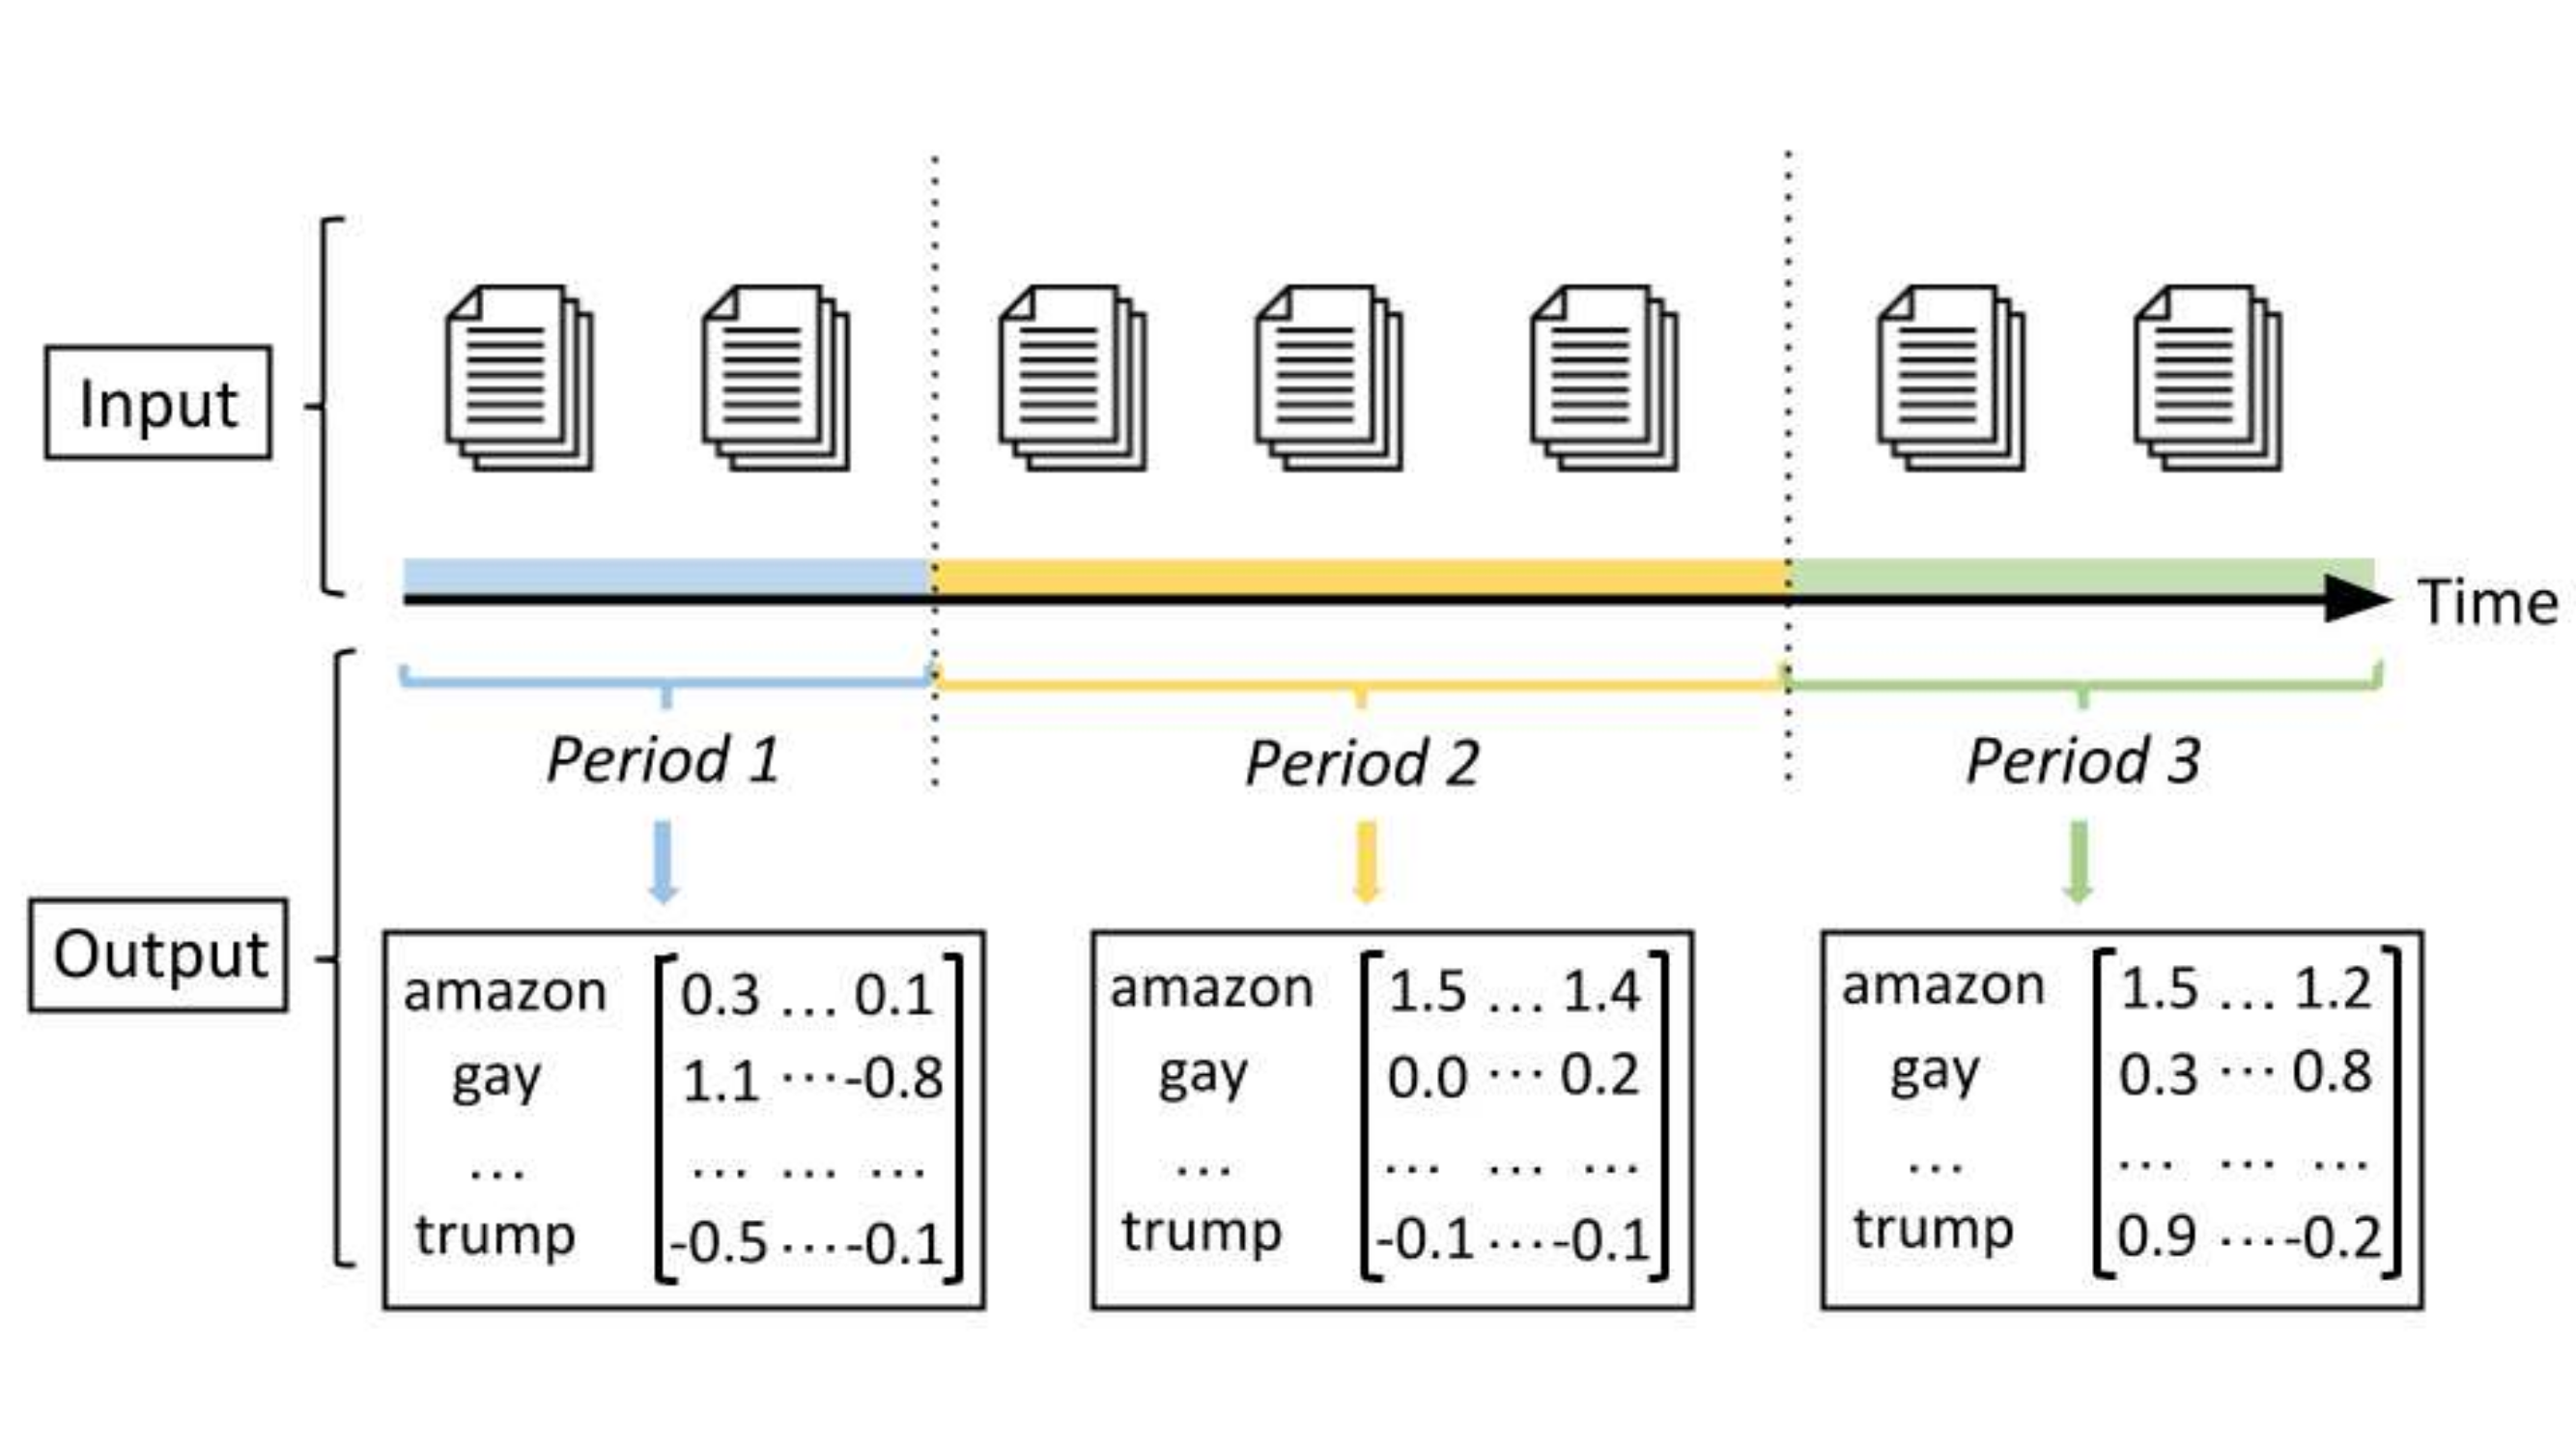
\includegraphics[width=1.0\textwidth]{figures/DUAN_overall.png}
\caption{Conceptual view of our task. Our goal is to identify latent periods in the input document collection, such that word semantics are relatively stable within the same period (i.e., a word is represented by the same embedding vector), and major linguistic shifts exist between different periods (i.e., a word may be represented by fairly different vectors in different periods).}\label{overall}
\end{figure}


The problem of document collection periodization based on evolving word semantics is however not trivial. In order to solve this problem, we address the following two research questions:\largerpage

\begin{enumerate}[label=\alph*.]
\item How to compute temporal-aware word embeddings?
\item How to split the document collection based on learned word embeddings?
\end{enumerate}

Our main technical contribution lies in a two-step framework for answering the above questions. First of all, we develop an anchor-based joint matrix factorization framework for computing time-aware word embeddings. More specifically, we concurrently factorize the time-stamped PPMI (positive pointwise mutual information) matrices, during which we utilize shared frequent terms (see Section \ref{Temporal word embeddings}) as anchors for aligning the word embeddings of each time frame to the same latent space. Furthermore, a block coordinate descent method is adopted to solve the learning model efficiently.
Secondly, we formulate the periodization task as an optimization problem, where we aim to maximize the aggregation of differences between the word semantics of any two periods. To solve this problem, we employ three classes of optimization algorithms which are based on greedy splitting, dynamic programming and iterative refinement, respectively. 

In the experiments, we use the crawled and publicly released New York Times dataset \citep{yao2018dynamic}, which contains a total of 99,872 articles published between January 1990 and July 2016. We compare the performance of our models with existing competitive temporal word embedding methods, and corpus periodization methods, respectively. 
To demonstrate the quality of our learned temporal word embeddings, we focus on the task of searching for temporal analogs (see Section \ref{embedding_effectiveness}).
To evaluate the periodization effectiveness, we construct the test sets by utilizing New York Times article tags (see Section \ref{periodization_effectiveness}), and evaluate the analyzed methods based on two standard metrics: Pk \citep{beeferman1999statistical} and WinDiff \citep{pevzner2002critique} used in text segmentation tasks.


In summary, our contributions are as follows:
\begin{itemize}
\item 
From a conceptual standpoint, we introduce a novel research problem of periodizing diachronic document collections for discovering the embodied evolutionary word semantics.
The discovered latent periods and corresponding temporal word embeddings can be utilized for many objectives, such as tracking and analyzing linguistic and topic shifts over time.
\item From a methodological standpoint, we develop an anchor-based joint matrix factorization framework for computing time-aware word embeddings, and three classes of optimization techniques for document collection periodization.
\item We perform extensive experiments on the New York Times corpus, which demonstrate the effectiveness of our approaches.
\end{itemize}

\section{Problem definition}\label{problem_definition}
We start by presenting the formal problem definition.

\subsection{Input} 
The input is a set of documents published across time. Each document is time-stamped and the whole text corpus spanning over a certain range of time is split into $N$ basic time frames $(t_{1}, t_{2}, ..., t_{N})$. The length of a time frame can be on the order of months, years, decades or centuries. Formally, let $D = \{D_{1}, D_{2}, ..., D_{N}\}$ denote the entire document set where $D_{x}, x = 1, ..., N$ represents the subset of documents belonging to the time frame $t_{x}$. 

\subsection{Task 1} 
Our first task is to find a $d$-dimensional embedding vector for each term in the overall corpus vocabulary $V = \{w_{1}, ..., w_{|V|}\}$,\footnote{The overall vocabulary $V$ is the union of vocabularies of each time unit, and thus it is possible for some $w \in V$ to not appear at all in some time units. This includes emerging words and dying words that are typical in real-world news corpora.} for each time unit $t_{i}, i = 1, ..., N$, respectively. We denote by $A_{i}$ the embedding matrix for $t_{i}$, whose $j$-th row represents the $d$-dimensional embedding vector of $j$-th term $w_{j}$ in $V$. Thus $A_{i}$ is of size $|V| \times d$. 

\subsection{Task 2} 
Based on Task 1, our second goal is to split the text corpus $D$ into $m$ contiguous, disjoint and coherent periods $\Theta =(P_{1}, P_{2}, ..., P_{m})$ and compute their corresponding word embedding matrices $E_{i}, i = 1, ..., m$. Note that in this study the value of $m$ is pre-defined. Each period $P_{i} = [\tau_{b}^{i}, \tau_{e}^{i}], i = 1, ..., m$ is expressed by two time points representing its beginning date $\tau_{b}^{i}$ and the ending date $\tau_{e}^{i}$, with $\tau_{b}^{1} = t_{1}$ and $\tau_{e}^{m} = t_{N}$. Let $L(\Theta) = (\tau_{b}^{1}, \tau_{b}^{2}, ..., \tau_{b}^{m})$ denote the list of beginning dates of $m$ periods, where $\tau_{b}^{1} = t_{1}$. Notice that searching for $\Theta$ is equivalent to discovering $L(\Theta)$. 

\section{Temporal word embeddings}
\label{Temporal word embeddings}

In this section, we describe our approach for computing dynamic word embeddings (solving Task 1 in Section \ref{problem_definition}), that captures lexical semantic dynamics across time.

\subsection{Learning static embeddings}
The distributional hypothesis \citep{firth1957} states that semantically similar words usually appear in similar contexts. Let $v_{i}$ denote the vector representing word $w_{i}$, then $v_{i}$ can be embodied in the co-occurrence statistics of $w_{i}$. In this study we first factorize the PPMI (positive pointwise mutual information) matrix for constructing static (i.e., time-agnostic) word embeddings, following previous works \citep{yao2018dynamic,levy2014neural,hamilton-etal-2016-diachronic}. 

For a corpus $D$ with vocabulary $V$, the $i,j$-th entry of PPMI matrix (of size $|V| \times |V|$) is given by

\begin{equation}\tag{1}
\begin{aligned}
\textup{PPMI}_{i,j} &= \textup{max}\left \{ \log_2\left ( \frac{p(w_{i},w_{j})}{p(w_{i})p(w_{j})} \right ), 0 \right \} \\&= \textup{max}\left \{ \log_2\left (\frac{c(w_{i}, w_{j})\cdot |D|}{c(w_{i})\cdot c(w_{j})}  \right ), 0 \right \}
\label{ppmi}
\end{aligned}
\end{equation}
where $p(w_{i},w_{j})$ represents the probability of words $w_{i}$ and $w_{j}$ co-occurring within a fixed-size sliding window of text, $c(w_{i},w_{j})$ counts the number of times that $w_{i}$ and $w_{j}$ co-occur, and $|D|$ is the total number of word tokens. Discarding the PPMI values under zero offers much better numerical stability \citep{yao2018dynamic}.

For word vectors $v_{i}$ and $v_{j}$, we should have $\textup{PPMI}_{i,j} \approx v_{i}\cdot v_{j}$, thus such word vectors can be obtained through factorizing the PPMI matrix.

\subsection{Learning dynamic embeddings}
\label{Learning dynamic embeddings}
In order to compute the embedding matrices $E = {E_{1}, ..., E_{m}}$ for a given segmentation $\Theta$ on corpus $D$, we first construct the embedding matrix $A_{i}, i = 1, ..., N$ for each time unit. We denote $\textup{PPMI}_{i}$ the PPMI matrix for time frame $t_{i}$, thus temporal word embeddings $A_{i}$ should satisfy $\textup{PPMI}_{i} \approx A_{i}\cdot A_{i}^{T}$. 


However, if $A_{i}$ is constructed separately for each time unit, due to the invariant-to-rotation nature of matrix factorization these learned word embeddings $A_{i}$ are non-unique (i.e., we have \[\textup{PPMI}_{i} \approx A_{i}\cdot A_{i}^{T} =  (A_{i}W^{T})\cdot (WA_{i}^{T}) = \tilde{A_{i}}\tilde{A_{i}^{T}}\] for any orthogonal transformation $W$ which satisfies $W^{T}\cdot W = I$). As a byproduct, embeddings across time frames may not be placed in the same latent space. Some previous works \citep{kulkarni2015statistically,hamilton-etal-2016-diachronic,zhang-etal-2015-omnia} solved this problem by imposing an alignment before any two adjacent matrices $A_{i}$ and $A_{i + 1}$, resulting in $A_{i} \approx A_{i + 1}, i = 1, ..., N - 1$.

Instead of solving a separate alignment problem for circumventing the non-unique characteristic of matrix factorization, we propose to learn the temporal embeddings across time concurrently. Note that for a word, we desire its vector to be close among all temporal embedding matrices, if it did not change its meaning across time (or change its meaning to very small extent). Such words are regarded as ``anchors" for connecting various embedding matrices, in our joint factorization framework. 

Essentially, we assume that very frequent terms (e.g., \textit{man}, \textit{sky}, \textit{one}, \textit{water}) did not experience significant semantic shifts as their dominant meanings are commonly used in everyday life and by many people. This assumption is reasonable as it has been reported in many languages including English, Spanish, Russian and Greek \citep{lieberman2007quantifying,pagel2007frequency}. We refer to these words as SFT, 
standing for \textsc{shared frequent terms}. 
Specifically, we denote by $A_{i}^{SFT}$ the $|V| \times d$ embedding matrix whose $i$-th row corresponds to the vector of word $w_{i}$ in $A_{i}$, if $w_{i}$ is a shared frequent term, and corresponds to zero vector otherwise, for a given time unit $t_{i}$. Our joint matrix factorization framework for discovering temporal word embeddings is then presented as follows (see Figure \ref{MF} for an illustration):\largerpage[-1]

\begin{equation}\tag{2}
\begin{aligned}
A_{1}, ..., A_{N} &= \operatorname{\underset{A}{argmin}}\sum_{i = 1}^{N}\left \|\textup{PPMI}_{i} - A_{i}\cdot A_{i}^{T}  \right \|_{F}^{2} \\&+ \alpha \cdot \sum_{i = 1}^{N}\left \| A_{i} \right \|_{F}^{2} + \beta \cdot \sum_{i = 1}^{N - 1}\sum_{j = i + 1}^{N}\left \| A_{i}^{SFT} -  A_{j}^{SFT}\right \|_{F}^{2}
\label{factorization}
\end{aligned}
\end{equation}

where the key smoothing term $\left \| A_{i}^{SFT} -  A_{j}^{SFT}\right \|_{F}^{2}$ aligns shared frequent terms in all years, thus places word embeddings across time in the same latent space. The regularization term $\left \| A_{i} \right \|_{F}^{2}$ is adopted to guarantee the low-rank data fidelity for overcoming the problem of overfitting. Parameters $\alpha$ and $\beta$ are used to control the weight of different terms to achieve the best factorization.

\iffalse
\begin{table}
\small
\centering
\caption{Examples of used Shared Frequent Terms.}
\label{sft_example}
\begin{tabular}{@{}c@{}}
\toprule
\begin{tabular}[c]{@{}c@{}}one, new, two, like, people,\\ year, many, women, time, company,\\ work, city, water, make, way,\\ use, world, business, school, life\end{tabular} \\ \bottomrule
\end{tabular}
\end{table}
\fi

\begin{figure}[ht]
\centering
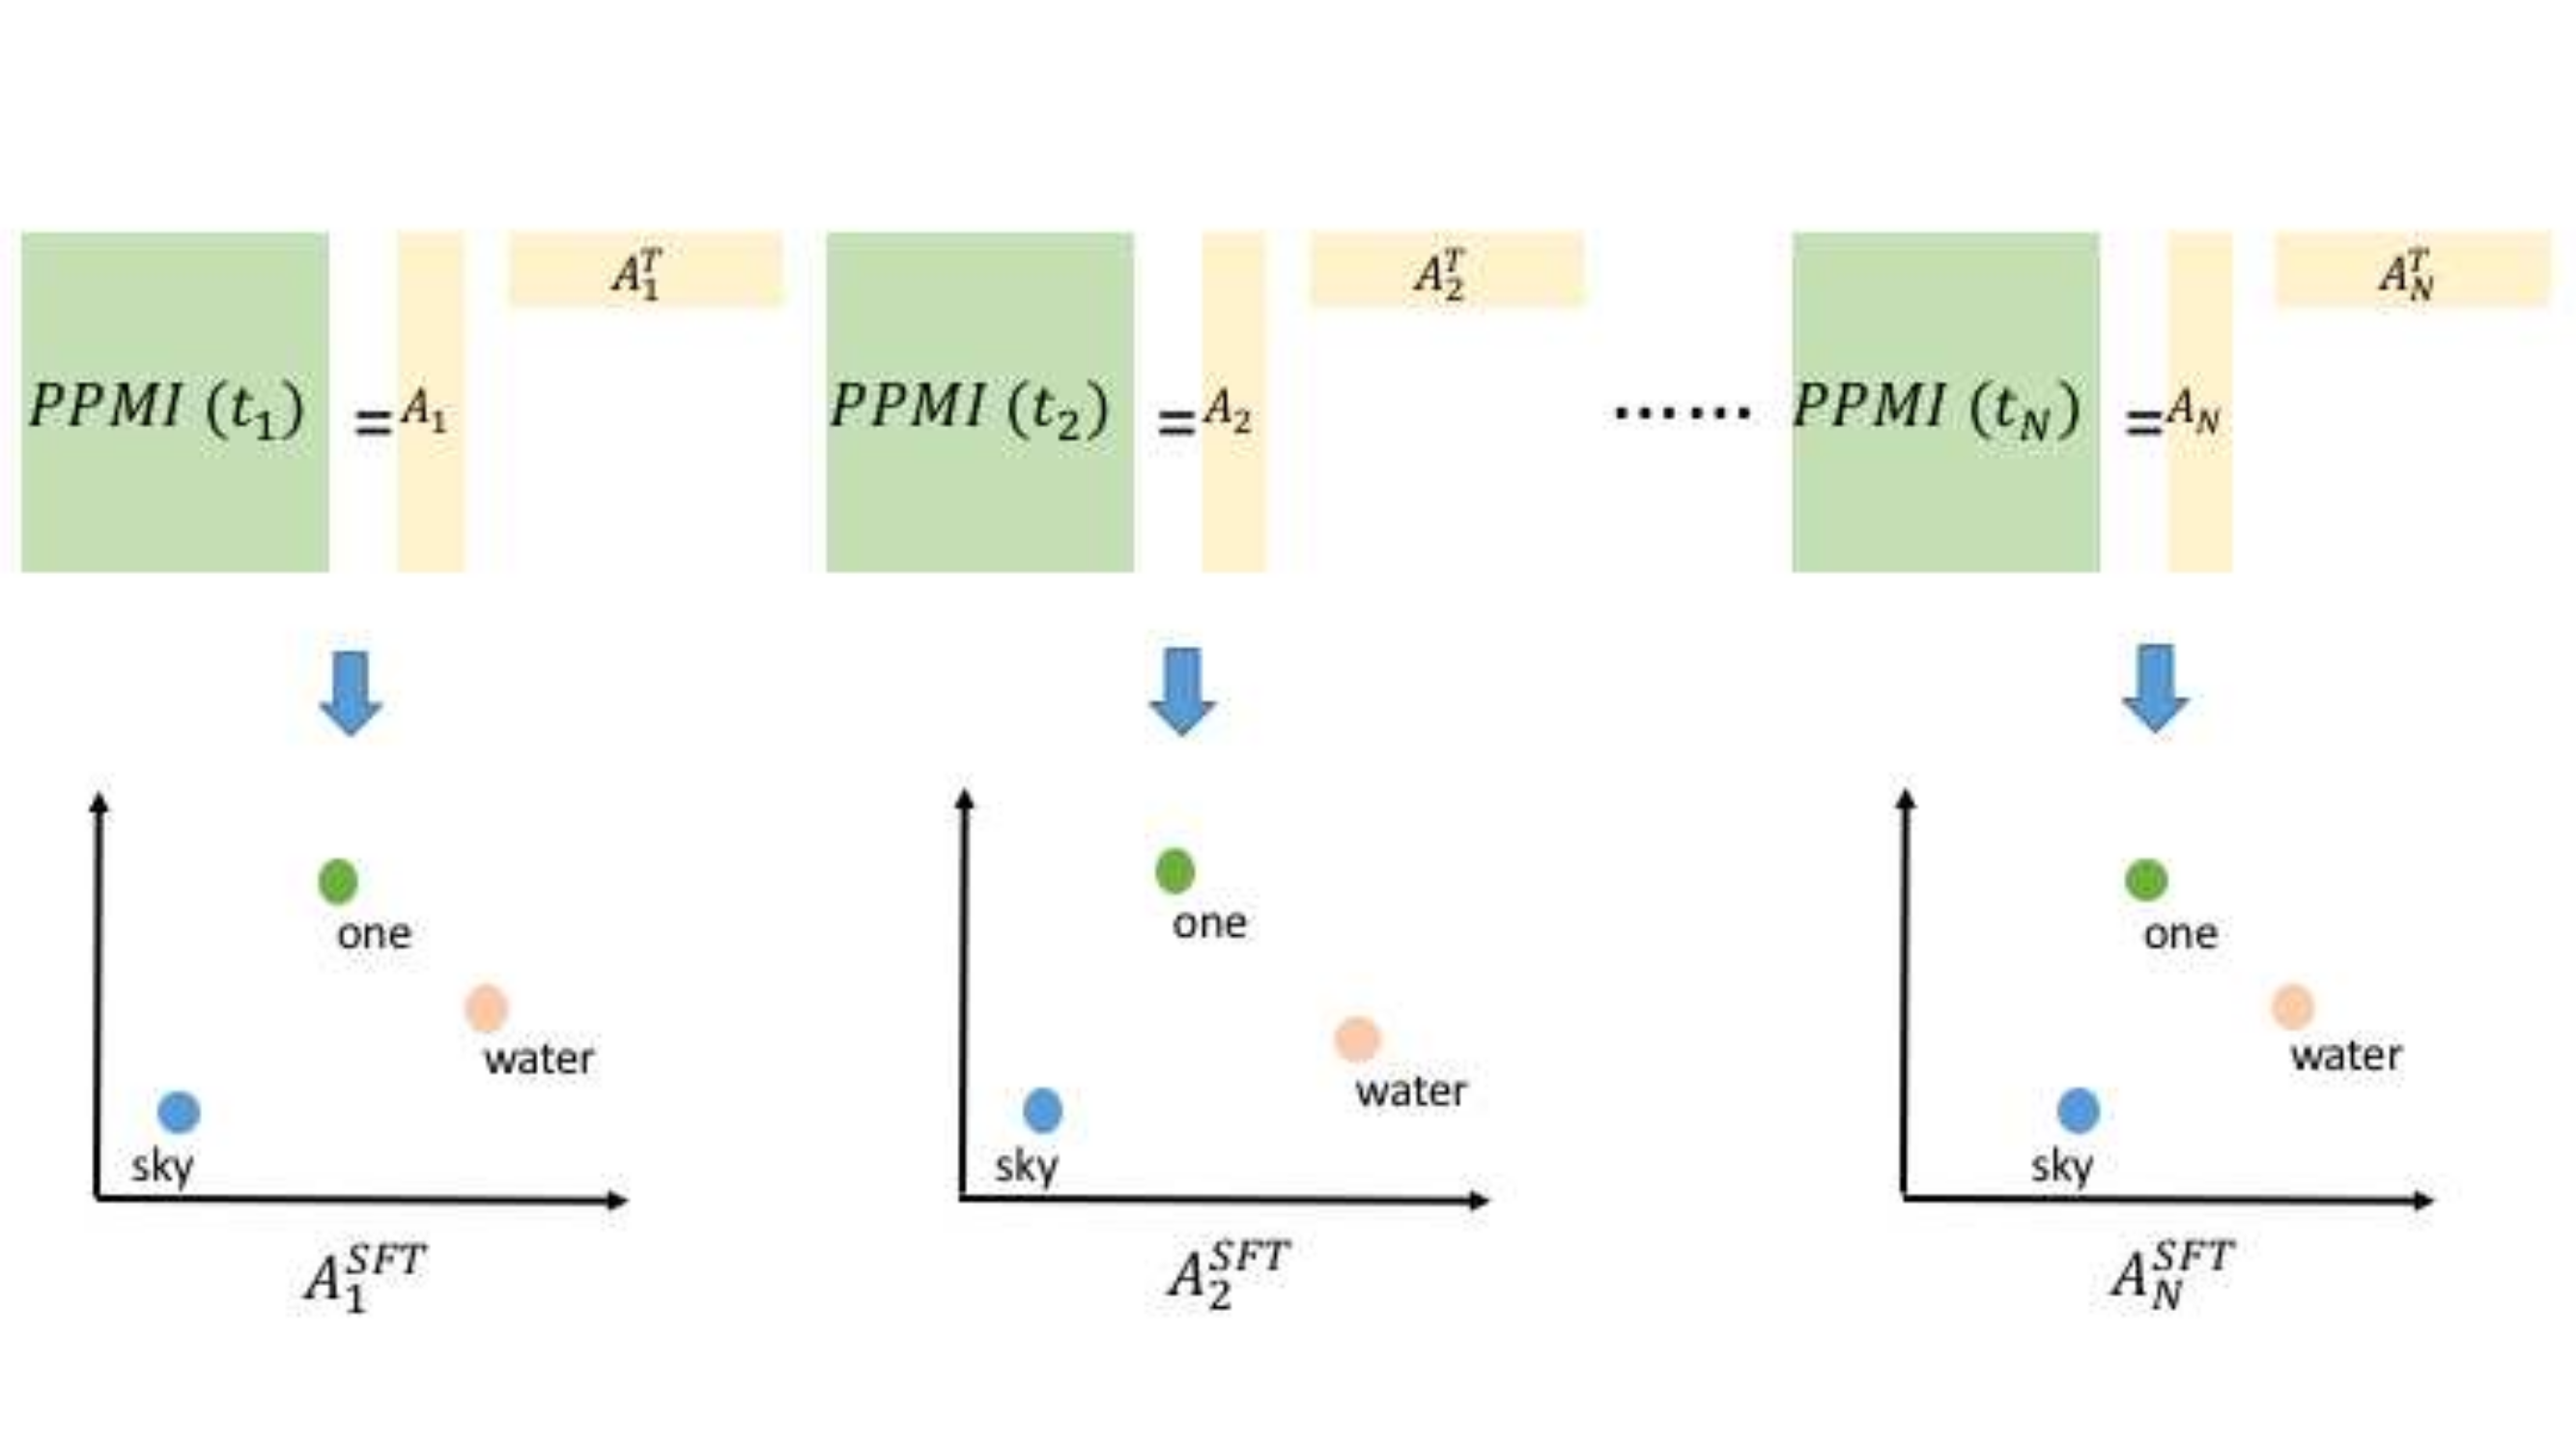
\includegraphics[width=0.9\textwidth]{figures/DUAN_mf.png}
\caption{Illustration of our joint matrix factorization model. Shared frequent terms in all time frames ($t_{1}, t_{2}, ..., t_{N}$) are aligned to similar positions, which places word embeddings across time in the same latent semantic space.}\label{MF}
\end{figure}

\subsection{Optimization}

The optimization problem in Equation \eqref{factorization} is not jointly convex to $A_{i}, i = 1, ..., N$, we first decompose the objective across periods, and solve for $A_{i}$ by fixing other embedding matrices as constants at each step. The problem of optimizing $A_{i}$ can be then formulated as follows:
\begin{equation}\tag{3}
\begin{aligned}
A_{i} = \operatorname{\underset{A}{argmin}}\ \Omega(A_{i}) &= \operatorname{\underset{A}{argmin}}\left \|\textup{PPMI}_{i} - A_{i}\cdot A_{i}^{T}  \right \|_{F}^{2} \\&+ \alpha \cdot \left \| A_{i} \right \|_{F}^{2} + \beta \cdot \sum_{j = 1}^{N}\left \| A_{i}^{SFT} -  A_{j}^{SFT}\right \|_{F}^{2}
\label{factorization_each_step}
\end{aligned}
\end{equation}

Notice that $\Omega(A_{i})$ is quartic in $A_{i}$, thus Equation \eqref{factorization_each_step} can not be optimized analytically. We then adopt the block coordinate descent \citep{tseng2001convergence} for iteratively minimizing $\Omega(A_{i})$. Specifically, the gradient of $\Omega(A_{i})$ with regard to $A_{i}$ is given by
\begin{equation}\tag{4}
\frac{\partial \Omega(A_{i}) }{\partial A_{i}} = 2(A_{i}\cdot A_{i}^{T} - \textup{PPMI}_{i} + \alpha)\cdot A_{i} + 2\beta \cdot \sum_{j = 1}^{N}(A_{i}^{SFT} - A_{j}^{SFT})
\label{gradient descent}
\end{equation}

where each above computation is of the order $O(\text{nnz}(\text{PPMI}_{i})d + d^{2}V)$ where $\text{nnz}(\text{PPMI}_{i})$ is the number of non-zeros in the matrix.

\section{Document collection periodization}

In this section, we prescribe how to obtain the final periods (solving Task 2 in Section \ref{problem_definition}). We first introduce the scoring objective of linguistic periodization, then we study the effectiveness of three optimization approaches: (1) greedy algorithm based periodization, which searches for the best available boundary at each step; (2) dynamic programming based periodization, which is able to discover the optimal periods in a dynamic programming manner; (3) an iterative refinement scheme, which iteratively refines the boundaries for improving the performance of the greedy strategy.

\subsection{Scoring}

To frame the periodization problem as a form of optimization, having built a particular segmentation $\Theta$, we now specify the way to quantify the quality of $\Theta$, and then adopt different classes of techniques to optimize that scoring objective. In general, we prefer the embedding matrices of different periods to be characterized by high inter-dissimilarity. More explicitly, the objective $\text{Obj}(\Theta)$ for an overall segmentation is given by aggregating the dissimilarity (expressed by the squared F-norm of the difference of two embedding matrices) between all pairs of period-specific embedding matrices, as follows:

%\begin{algorithmic}
\begin{equation}\tag{5}
\text{Obj}(\Theta) = \text{Obj}(L(\Theta)) = \sum_{i = 1}^{m - 1} \sum_{j = i + 1}^{m}\left \| E_{i} - E_{j} \right \|_{F}^{2}
\label{objective}
\end{equation}

Here, $m$ is the pre-defined number of periods. $E_{i}$ is measured as the average of embeddings $A_{t}$ for time unit $t$ in period $P_{i} = [\tau_{b}^{i}, \tau_{e}^{i}]$, as follows:
\begin{equation}\tag{6}
E_{i} = \frac{1}{\tau_{e}^{i} - \tau_{b}^{i} + 1}\sum_{t = \tau_{b}^{i}}^{\tau_{e}^{i}}{A_{t}}
\label{period_embedding}
\end{equation}
The segmentation that achieves the highest score of Equation \eqref{objective} will be adopted.

\subsection{Periodizing}
\label{periodization_algorithms}

\subsubsection{Greedy algorithm based periodization}

The greedy periodization algorithm is not guaranteed to reach the optimal splitting, however it offers significant computational benefit. At each step, it greedily inserts a new boundary (which is the beginning date of a new period) to the existing segmentation to locally maximize the objective function, until desired $m$ periods are discovered. The process of greedy periodization is formulated as follows:
\begin{equation}\tag{7}
L(\Theta)^{i + 1} = \underset{t_{p} \in \left [ t_{1}, t_{N} \right ], t_{p} \notin L(\Theta)^{i}}{\textup{arg max}\ \text{Obj}(L(\Theta)^{i} \cup \left \{ t_{p} \right \})}
\label{greedy}
\end{equation}

where $L(\Theta)^{i}$ denotes the list of boundaries (or the beginning dates of periods) at the $i$-th step, and $L(\Theta)^{0} = \{t_{1}\}$. The process of greedy algorithm based periodization is shown in Algorithm 1.

\begin{algorithm}
\SetAlgoLined
\SetKwInOut{Input}{input\,}
\SetKwInOut{Output}{output\,}
\SetKw{Continue}{continue}
\Input{$L(\Theta)^{0}$; $m$}
\Output{$L(\Theta)^{m - 1}$}
\For{$i \leftarrow 0$ \KwTo $m - 2$}{
$max\_score \leftarrow 0$\;
$next\_boundary \leftarrow 0$\;
\For{$t_{p} \leftarrow t_{1}$ \KwTo $t_{N}$}
{
\Comment*[h]{~Find the best local boundary}\;
\If{$t_{p} \in L(\Theta)^{i}$}{
\Continue
}
$score \leftarrow \text{Obj}(L(\Theta)^{i} \cup \left \{ t_{p} \right \})$\;
\If{$score > max\_score$}{
   $max\_score \leftarrow score$\;
   $next\_boundary \leftarrow t_{p}$\;
   }
}
$L(\Theta)^{i + 1} \leftarrow L(\Theta)^{i} \cup \left \{next\_boundary \right \}$\;
}
\caption{Greedy algorithm based periodization}
\end{algorithm}

\subsubsection{Dynamic programming based periodization}

The core idea of dynamic programming based periodization is to break the overall problem into a series of simpler smaller segmentation tasks, and then recursively find the solutions to the sub-problems. By recursively solving the sub-problems optimally, the dynamic programming approach yields the globally optimal value of Equation \eqref{objective}. Let $\Theta^{l}_{k}$ denote the segmentation of the first $l$ time slices of the entire time span into $k$ periods. The computational process of dynamic programming based periodization is then expressed as follows:
\begin{equation}\tag{8}
L(\Theta^{N}_{k}) = \underset{l < N}{\textup{arg max}\ \text{Obj}(L(\Theta^{l}_{k-1})\cup t_{l + 1})}
\label{dp}
\end{equation}

where $\Theta^{l}_{1} = [t_{1}, t_{l}]$ and $L(\Theta^{l}_{1}) = \{t_{1}\}, l = 1, ..., N$. In practice, though each of those sub-problems can be solved in one pass by storing their solutions in a memory-based data structure (array, map, etc), the dynamic programming approach can be costly to compute, compared to the greedy splitting, as shown below in Section~\ref{sec:08-analysis-time-complexity}. The process of dynamic programming based periodization is shown in Algorithm 2.

\begin{algorithm}
\SetAlgoLined
\SetKwInOut{Input}{input\,}
\SetKwInOut{Output}{output\,}
\SetKw{Continue}{continue}
\Input{L($\Theta^{l}_{1}$), $l = 1, ..., N$; $m$}
\Output{$L(\Theta^{N}_{m})$}
\For{$row \leftarrow 2$ \KwTo $m$}
{
\For{$col \leftarrow row$ \KwTo $N$}
{
\Comment*[h]{~Recursively find the solutions to the sub-problems}\;
$max\_score \leftarrow 0$\;
$next\_boundary \leftarrow 0$\;
$subtask \leftarrow 0$\;
\For{$j \leftarrow row - 1$ \KwTo $col - 1$}
{
$score \leftarrow \text{Obj}(L(\Theta^{j}_{row - 1}) \cup \left \{ t_{j + 1} \right \})$\;
\If{$score > max\_score$}{
   $max\_score \leftarrow score$\;
   $next\_boundary \leftarrow t_{j + 1}$\;
   $subtask \leftarrow j$\;
   }
}
$L(\Theta^{col}_{row}) \leftarrow L(\Theta^{subtask}_{row - 1}) \cup \left \{ next\_boundary \right \}$
}
}
\caption{Dynamic programming based periodization}
\end{algorithm}

\subsubsection{Iterative refinement based periodization}

The iterative refinement framework starts with the greedy segmentation. At each step after the best available boundary is found, a relaxation scheme which tries to adjust each segment boundary optimally while keeping the edges (i.e. adjacent boundaries) to either side of it fixed, is applied. This method can improve the performance of the greedy scheme, while at the same time retain its computational benefit to some extent.
Let $L(\Theta)^{i}_{G}[j]$ denote the $j$-th element in $L(\Theta)^{i}$ after the $i$-th greedy search step, the iterative refinement process for finding $L(\Theta)^{i}[j]$ is shown as follows:
\begin{equation}\tag{9}
L(\Theta)^{i}[j] = \underset{t_{p} \in \left ( L(\Theta)^{i}[j - 1], L(\Theta)^{i}[j + 1] \right )}{\textup{arg max}\ \text{Obj}((L(\Theta)^{i} \setminus {L(\Theta)^{i}_{G}[j]})\cup \left \{ t_{p} \right \})}
\label{iterative_1}
\end{equation}

The process of this method is shown in Algorithm 3 below.
\begin{algorithm}
\SetAlgoLined
\SetKwInOut{Input}{input\,}
\SetKwInOut{Output}{output\,}
\SetKw{Continue}{continue}
\Input{$L(\Theta)^{0}$; $m$}
\Output{$L(\Theta)^{m - 1}$}
\For{$i \leftarrow 0$ \KwTo $m - 2$}
{
$next\_boundary, max\_score \leftarrow Greedy(L(\Theta)^{i})$\;
$L(\Theta)^{i + 1} \leftarrow L(\Theta)^{i} \cup \left \{ next\_boundary \right \}$\;
\For{$j \leftarrow 1$ \KwTo $i$}{
\Comment*[h]{~Iteratively refine the previous boundaries}\;
$new\_boundary \leftarrow L(\Theta)^{i + 1}[j]$\;
$t_{begin} \leftarrow L(\Theta)^{i + 1}[j - 1]$\;
$t_{end} \leftarrow L(\Theta)^{i + 1}[j + 1]$\;
\For{$t_{p} \leftarrow t_{begin}$ \KwTo $t_{end}$}{
$score \leftarrow \text{Obj}(L(\Theta)^{i + 1} - {L(\Theta)^{i + 1}[j]}\cup \left \{ t_{p} \right \})$\;
\If{$score > max\_score$}{
   $max\_score \leftarrow score$\;
   $next\_boundary \leftarrow t_{p}$\;
}
}
$L(\Theta)^{i + 1} \leftarrow (L(\Theta)^{i + 1} - {L(\Theta)^{i + 1}[j]})\cup \left \{ new\_boundary \right \}$\;
}
}
\caption{Iterative refinement based periodization}
\end{algorithm}

\subsection{Analysis of time complexity}\label{sec:08-analysis-time-complexity}
For greedy periodization, it requires $m - 1$ steps and the $i$-th step calls the scoring function Equation \eqref{objective} $N - i$ times. In total, it is $Nm - N - m^{2} + m/2$. In the case of $N \gg m$, the greedy periodization algorithm takes $O(Nm)$. For dynamic programming based periodization, it requires $O(Nm)$ states and evaluating each state involves an $O(N)$ calling of Equation \eqref{objective}. Then the overall algorithm would take $O(N^{2}m)$. Finally, for iterative refinement based periodization, an upper bound on its time complexity is $O(\sum_{i = 1}^{m - 1}(N - i)*i)$ = $O(Nm^{2})$.

\section{Embedding effectiveness}
\label{embedding_effectiveness}
\subsection{Datasets}
\label{datasets}
News corpora, which maintain consistency in narrative style and grammar, form a good basis for studying language evolution.
We perform the experiments on the New York Times Corpus, which has been frequently used to evaluate different researches that focus on temporal information processing or extraction in document archives \citep{campos2014survey}. 
The dataset we use \citep{yao2018dynamic} is a collection of 99,872 articles published by the New York Times between January 1990 and July 2016. For the experiments, we first divide this corpus into 27 frames, setting the length of time unit to be 1 year. Stopwords and rare words (which have less than 200 occurrences in the entire corpus) were removed before experiments, following  previous work \citep{zhang-etal-2015-omnia}.
The statistics of our dataset are shown in Table \ref{nyt}.

\begin{table}
\caption{Summary of the New York Times dataset\label{nyt}}
\fittable{
\begin{tabular}{ccccc}
\lsptoprule
\#Articles & \#Vocabulary & \#Word Co-occurences & \#Time units & Range\\\midrule
99,872     & 20,936              & 11,068,100       & 27            & Jan. 1990--Jul. 2016 \\ 
\lspbottomrule
\end{tabular}
}
\end{table}

\subsection{Experimental settings}
\label{settings}

We describe next the parameters used in the experiments. 
For the construction of the PPMI matrix, the length of the sliding window and the embedding dimensions is set to be 5 and 50, respectively, following \citep{yao2018dynamic}. During the training process, the values of  parameters $\alpha$ and $\beta$ (see Equation \eqref{factorization}) are set to be 20 and 100, respectively, as the result of a grid search. The selection of shared frequent terms (see Section \ref{Learning dynamic embeddings}) used as anchors is set to be the top 5\% most popular words in the entire corpus excluding stopwords, as suggested by \citep{zhang-etal-2015-omnia}.

\subsection{Compared methods}
We describe here the analyzed methods for learning temporal word embeddings.

\begin{description}
\item[Without transformation (Non-Tran):] This method directly compares the vectors in different time without performing any transformation.

\item[Linear transformation (LT) \citep{zhang-etal-2015-omnia}:] The embeddings are first trained separately for each year, and then are transformed by optimizing a linear transformation between adjacent years. 

\item[Orthogonal transformation (OT) \citep{hamilton-etal-2016-diachronic}:] The embeddings are first trained separately for each year, and then are aligned by optimizing an orthogonal transformation between adjacent years.

\item[Dynamic Word2Vec (DW2V) \citep{yao2018dynamic}:] The embeddings are trained based on PPMI matrices by minimizing the distance between embeddings in only adjacent years, without using SFTs.

\item[The proposed model (this paper):] The embeddings are jointly learned, by minimizing the difference between embeddings of shared frequent terms within the entire period.
\end{description}

We use the publicly available source code released by \citep{yao2018dynamic} for all baseline methods.\footnote{\url{https://github.com/yifan0sun/DynamicWord2Vec}}

\subsection{Test sets}

To demonstrate the effectiveness of our model, we focus on the task of searching for temporal analogs. 
We utilize 2 testsets \citep{yao2018dynamic} containing queries in the base time (e.g., \textit{obama} in 2012) and their analogs in target time (e.g., \textit{bush} in 2002).
Testset 1 includes publicly recorded knowledge that for each year lists different names for a particular role (e.g., U.S. president),\footnote{Note that we find several mistakes in this testset, such as (\textit{pistons-1990, knicks-1999}) (the correct pair should be (\textit{pistons-1990, spurs-1999})). Then we manually correct them and use the corrected version for all analyzed methods in experiment.} and testset 2 consists of interesting concepts such as emerging technologies, brands and major events (e.g., \textit{app} in 2012 can correspond to \textit{software} in 1990: \citealp{yao2018dynamic}).
In total, there are 11,473 pairs of terms (query and its analog) used in our experiments.

\subsection{Evaluation metrics}
The \textsc{mean reciprocal rank} (MRR) is used for evaluating the search results for each learning model, which is computed as follows:

\begin{equation}\tag{10}
\text{MRR} = \frac{1}{N}\sum_{i = 1}^{N}\frac{1}{\textit{rank}_{i}}
\end{equation}

where $\textit{rank}_{i}$ is the rank of a correct temporal analog at the $i$-th test, and $N$ is the number of test pairs.

In addition, precisions @1, @5, @10 and @20 are also reported. Those metrics refer to the rates of tests in which the correct temporal analog was included in the top 1, 5, 10 and 20 results, respectively. All the values of used metrics fall into [0,1]. The higher the values are, the more effectively a model works.

\subsection{Experimental results}
\begin{table}\footnotesize
\caption{Performance of all analyzed models for learning dynamic word embeddings.\label{RQ1}}
\fittable{
\begin{tabular}{lcccccccccc}
\lsptoprule
            & \multicolumn{5}{c}{Testset 1}         & \multicolumn{5}{c}{Testset 2}               \\\cmidrule(lr){2-6}\cmidrule(lr){7-11}
            & MRR & P@1 & P@5 & P@10 & P@20 & MRR & P@1 & P@5 & P@10 & P@20 \\\midrule
Non-Tran        &          0.012&         0.020&    0.034     &         0.042&          0.064&0.005         &0.000         &0.000         &0.018         &0.025          \\
LT         &         0.137&         0.118&         0.232&         0.267&          0.355&        0.038&         0.021&         0.065&         0.146&          0.219\\
OT         &         0.158&         0.106&         0.224&         0.295&          0.373&         0.050&         0.023&         0.079&         0.142&          0.185\\
DW2V         &         0.422&         0.331&         0.549&         0.619&          0.703&         0.144&         0.076&         0.220&         0.382&          0.487\\
Our model     &         0.454&         0.348&         0.563&         0.651&          0.740&         0.157&         0.082&         0.255&         0.406&   0.520          
\\\lspbottomrule
\end{tabular}
}
\end{table}

Table \ref{RQ1} shows the scores for all the methods averaged on all the tested queries on testset 1 and testset 2, respectively. We first notice that the performance is extremely poor without transforming the contexts of queries. The correct answers in the Non-Tran approach are usually found at ranks $>$ 1k which is in line with observations made by \citet{zhang-etal-2015-omnia}. 
On the other hand, both transformation-based methods LT and OT are helpful since they exhibit significantly better effectiveness compared to Non-Tran. This observation suggests little overlap in the contexts of news articles which are separated by long time gaps, and that the task of temporal analog identification is quite difficult.
Moreover, it is evident that learning the temporal embeddings across time by enforcing a global alignment is superior to following the ``separately learning-and-aligning'' pattern, since both DW2V and our approach outperform LT and OT significantly. Therefore, enforcing a global alignment is more effective for solving the temporal analog detection task.

Lastly, a closer look at Table \ref{RQ1} reveals that regardless of the type of evaluation metric, our model improves upon the performance of the state-of-the-art DW2V model. Specifically, our method improves DW2V model by 9.0\% and 7.6\% when measured using the main metric MRR on testset 1 and testset 2, respectively. The plausible reason is that DW2V does not differentiate words with stable meanings from words whose semantics are evolving, while such assumption may lead to a less precise learned representation of words. By injecting additional knowledge of shared frequent terms as anchors, our approach allows for only aligning embeddings of such stable words, and keeping the representation of other words exactly as their diachronic contexts express.

\section{Periodization effectiveness}
\label{periodization_effectiveness}

\subsection{Datasets}
We use the same news article datasets as described in Section \ref{datasets}.

\subsection{Compared methods}
We implemented below two types of periodization models as analyzed methods (proposed methods and baselines) in order to compare the periods they generate with the reference periods.

\subsubsection{Baseline methods} 
We test four baselines as listed below.
\begin{description}\sloppy
\item[Random:] The segment boundaries are randomly inserted.
\item[VNC \citep{gries2012variability}:] A bottom-up hierarchical variability-based neighbor clustering (VNC) approach to periodization.
\item[KLD \citep{degaetano2018using}:] An entropy-driven approach which calculates the Kullback-Leibler Divergence (KLD) between term frequency features in text from temporally adjacent time periods to identify stages of language change.
\item[CPD \citep{kulkarni2015statistically}:] An approach which uses statistically sound change point detection (CPD) algorithms to detect significant linguistic shifts based on mean shift model.
\end{description}

\subsubsection{Proposed methods}
 We list three proposed methods below  (see Section \ref{periodization_algorithms}).

These proposed methods adopt different strategies to optimize Equation \eqref{objective}, based on the temporal word embeddings obtained in Section \ref{Temporal word embeddings}.

\begin{description}
\item[G-WSE:] Greedy periodization based on word semantic evolution. 
\item[DP-WSE:] Dynamic programming periodization based on word semantic evolution. 
\item[IR-WSE:] Iterative refinement based on word semantic evolution.
\end{description}

\subsection{Test sets}
As far as we know there are no standard testsets for New York Time Corpus. We therefore had to create test sets. Note that the collected news articles dataset is associated with some metadata, including title, author, publication time, and topical section label (e.g., \textit{Science}, \textit{Sports}, \textit{Technology}) which describes the general topic of news articles. Such section labels could be used to locate the boundaries of word meanings.

Intuitively, if a word $w$ is strongly related to a particular section $s$ in year $t$, we associate $w$, $s$ and $t$ together and construct a $\langle w, s, t\rangle$ triplet. A boundary of $w$ is registered if it is assigned to different sections in two adjacent years (i.e., both triplet $\langle w, s, t\rangle$ and $\langle w, s', t + 1\rangle$ hold and $s \neq s'$).

More specifically, for each word $w$ in the corpus vocabulary $V$ we compute its frequency in all sections for each year $t$, and $w$ is assigned to the section in which $w$ is most frequent. Note that this word frequency information is not used in our learning model. In this study we utilize the 11 most popular and discriminative sections of the New York Times,\footnote{These sections are \textit{Arts}, \textit{Business}, \textit{Fashion \& Style}, \textit{Health}, \textit{Home \& Garden}, \textit{Real Estate}, \textit{Science}, \textit{Sports}, \textit{Technology}, \textit{U.S.}, \textit{World}.} following previous work \citep{yao2018dynamic}.

Recall that parameter $m$ denotes the number of predefined latent periods. For each different $m$, we first identify the set of words $S_{m}$ characterized by the same number of periods. Then for each method and each value of $m$, we test the performance of such method by comparing the generated periods with the reference segments of each word in $S_{m}$, and then take the average. In this study, we experiment with the variation in the value of $m$, ranging from 2 to 10.

\subsection{Evaluation metrics}

We evaluate the performance of the analyzed methods with respect to two standard metrics: Pk \citep{beeferman1999statistical} and WinDiff \citep{pevzner2002critique} used in text segmentation tasks. Both metrics use a sliding window of fixed size $k$ over the document and compare the newly generated segments with the reference ones. Here $k$ is generally set as follows \citep{beeferman1999statistical}:

\begin{equation}\tag{11}
k = \left\lfloor\frac{\#time \ units}{2\cdot \#periods}\right\rfloor - 1
\end{equation}

Specifically, the Pk metric counts the number of disagreements on the probe elements as follows:

\begin{equation}\tag{12}
\text{Pk} = \frac{1}{N - k}\sum_{i = 1}^{N - k}[P_{\text{hyp}}(i, i + k) \neq P_{\text{ref}}(i, i + k)]
\end{equation}

where $N$ indicates the number of elements (in our case, the number of time units) and $P(i, i + k)$ is equal to 1 or 0 according to whether or not both element $i$ and $i + k$ are recognized as being in the same segment in hypothesized segmentation $P_{\text{hyp}}$ and reference segmentation $P_{\text{ref}}$. Since Pk metric has the disadvantage that it penalizes false positives more severely than false negatives \citep{alemi2015text}, the WinDiff metric was introduced. It is defined as follows:

\begin{equation}\tag{13}
\text{WinDiff} = \frac{1}{N - k}\sum_{i = 1}^{N - k}[W_{\text{hyp}}(i, i + k) \neq W_{\text{ref}}(i, i + k)]
\end{equation}

where $W_{\text{hyp}}(i, i + k)$ and $W_{\text{ref}}(i, i + k)$ each count the number of boundaries between the time units $i$ and $i + k$ in generated and reference segments, respectively. An error is registered if they are different. Both Pk and WinDiff give values in the range [0, 1]. They are equal to 0 if and only if an algorithm assigns all boundaries correctly. The lower the scores are, the better the algorithm performs. 

\subsection{Evaluation results}
Tables~\ref{pk} and~\ref{windiff} summarize the Pk and WinDiff scores for each method, respectively. Based on the experimental data we make the following observations.

\begin{itemize}
\item The proposed methods exhibit the overall best performance regarding both Pk and WinDiff metrics. More specifically, they outperform the best baseline under 7 of 9 predefined numbers of periods in terms of Pk, and 6 of 9 in terms of WinDiff. 
This demonstrates the effectiveness of our proposed periodization frameworks.
\item Regarding baseline methods, Random achieves the worst performance as expected. CPD and KLD show competitive performance under certain settings. CPD gets two wins in terms of Pk, and KLD obtains three wins in terms of WinDiff.
\item DP-WSE is the best performer among all three proposed periodization algorithms.
It contributes 6 best performance in terms of Pk, and 5 in terms of WinDiff.
Moreover, when compared to G-WSE and IR-WSE, DP-WSE shows a 3.79\% and 3.24\% increase in terms of Pk, and a 7.77\% and 6.46\% increase in terms of WinDiff, respectively. 
This observation is in good agreement with the theoretical analysis, which states that dynamic programming based segmentation sacrifices computational efficiency for the optimal splitting.
\item The operation of iterative refinement indeed improves the performance of greedy periodization. However, the improvement is marginal: many results generated by IR-WSE are similar or identical to those from G-WSE.
\end{itemize}



\begin{table}
\small
\caption{Performance comparison using Pk (Lower scores indicate better performance).}
\label{pk}
\centering
\begin{tabular}{cccccccccc}
\lsptoprule
\multirow{2}{*}{Acronym} & \multicolumn{9}{c}{Number of periods}\\ \cmidrule(lr){2-10} 
                                                                           & 2              & 3              & 4              & 5              & 6              & 7              & 8              & 9              & 10             \\ \midrule
Random                   & 0.467          & 0.474          & 0.545          & 0.522          & 0.542          & 0.480          & 0.480          & 0.480          & 0.539          \\  
                                                  VNC                      & 0.385          & 0.253          & 0.249          & 0.290          & 0.282          & 0.302          & 0.302          & 0.294          & 0.303          \\  
                                                  KLD              & 0.385          & 0.278          & 0.244          & 0.270          & 0.276          & 0.278          & 0.284          & 0.290          & 0.304          \\  
                                                  CPD                 & 0.238          & 0.234          & 0.246          & 0.260          & 0.282          & 0.263 & 0.249 & 0.299          & 0.338          \\ 
G-WSE                   & 0.115 & 0.201 & 0.248          & 0.282          & 0.300          & 0.310          & 0.312          & 0.292          & 0.303          \\  
                                                  DP-WSE                  & 0.115 & 0.230          & 0.236 & 0.251 & 0.271 & 0.290          & 0.291          & 0.286 & 0.296 \\  
                                                  IR-WSE                  & 0.115 & 0.201 & 0.244
                                                 & 0.279          & 0.300          & 0.304          & 0.312          & 0.292          & 0.303          \\ \lspbottomrule
\end{tabular}
\end{table}

\begin{table}
\small
\caption{Performance comparison using WinDiff (Lower scores indicate better performance).}
\label{windiff}
\centering
\begin{tabular}{cccccccccc}
\lsptoprule
\multirow{2}{*}{Acronym} & \multicolumn{9}{c}{Number of periods}                                                                                                                 \\ \cmidrule(lr){2-10} 
                                                                                       &2                                   & 3              & 4              & 5              & 6              & 7              & 8              & 9              & 10             \\ \midrule
Random                   & 0.467                               & 0.474          & 0.545          & 0.478          & 0.542          & 0.480          & 0.480          & 0.480          & 0.500          \\ VNC                      & 0.417                               & 0.346          & 0.396          & 0.416          & 0.426          & 0.434          & 0.439          & 0.435          & 0.388          \\KLD              & 0.417                               & 0.343          & 0.383          & 0.384 & 0.428          & 0.437          & 0.434          & 0.430         & 0.384         \\CPD                 & 0.414                               & 0.386          & 0.387          & 0.394          & 0.430          & 0.430          & 0.430          & 0.432          & 0.385          \\ 
G-WSE                   & 0.383                      & 0.430          & 0.435          & 0.449          & 0.456          & 0.449          & 0.447          & 0.432          & 0.387          \\ DP-WSE                  & 0.383                      & 0.336 & 0.387          & 0.403          & 0.423 & 0.422 & 0.430          & 0.431          & 0.388          \\IR-WSE                  & 0.383                  & 0.405          & 0.428          & 0.449          & 0.456          & 0.449          & 0.447          & 0.421 & 0.387          \\ \lspbottomrule
\end{tabular}
\end{table}
\section{Related work}

\subsection{Text segmentation}
The most similar task to the document collection periodization is text segmentation. The task of text segmentation is formulated as splitting a chunk of text into meaningful sections based on their topic continuity, and it has many useful applications in information retrieval, text summarization, etc. Early text segmentation approaches include TextTiling \citep{hearst1997texttiling} and the C99 algorithm \citep{choi2000advances}, which are based on some heuristics on text coherence using a bag of words representation. Furthermore many attempts adopt topic models to inform the segmentation task, including \citet{riedl2012text,du2013topic}. \citet{alemi2015text} is a segmentation algorithm based on time-agnostic semantic word embeddings. Most text segmentation methods are unsupervised. However, neural approaches have also been explored for domain-specific text segmentation tasks, such as \citet{sehikh2017topic}.
Many text segmentation algorithms are greedy in nature, such as \citet{choi2000advances,choi2001latent}. Moving beyond the greedy approach, some works search for the optimal splitting for their own objective using dynamic programming \citep{utiyama2001statistical,fragkou2004dynamic}. 

Apart from computer scientists, social scientists also have proposed a variety of methods to break a corpus into coherent sections. Related frameworks include those of \citet{ruef1999social,th2008identification,alsudais2016corpus}. Some studies are investigating the temporal topics in various corpora including news \citep{allan2001temporal}, historical documents \citep{duan2017discovering} or scientific archives \citep{blei2006dynamic,topicsovertime}.

\subsection{Temporal word embeddings}
How to best represent words with low-dimensional dense vectors has attracted consistent interest for several decades. Early methods are relying on statistical models \citep{lund1996producing,blei2003latent}, while in recent years neural models such as word2vec \citep{mikolov2013efficient} and GloVE \citep{pennington-etal-2014-glove} have shown great success in many NLP applications. Moreover, it has been demonstrated that both word2vec and GloVE are equivalent to factorizing the PMI matrix \citep{levy2014neural}, which motivates our approach.

The above methods assume word representation is time-agnostic. Recently some works explored computing time-aware embeddings of words, for analyzing linguistic change and evolution \citep{yao2018dynamic,zhang-etal-2015-omnia,hamilton-etal-2016-diachronic,kulkarni2015statistically,wordsaremalleable,gonen2020simple}. In order to compare word vectors across time most works ensure the vectors are aligned to the same coordinate axes, by solving the least squares problem \citep{zhang-etal-2015-omnia,kulkarni2015statistically}, imposing an orthogonal transformation \citep{hamilton-etal-2016-diachronic} or jointly smoothing every pair of adjacent time slices \citep{yao2018dynamic}. Different from the existing methods, in this study we inject additional knowledge by using shared frequent terms as anchors to simultaneously learn the temporal word embeddings and circumvent the alignment problem.

\section{Conclusion}
This work approaches a novel task -- diachronic document collection periodization. The special character of our task allows capturing evolutionary word semantics.
The discovered latent periods can be an effective indicator of linguistics shifts and evolution embodied in analyzed diachronic textual corpora. To address the introduced problem we propose a two-step framework which consists of 
a joint matrix factorization model for learning dynamic word embeddings, and a well-defined optimization formulation for corpus periodization.
For solving the resulting optimization problem we develop a series of effective algorithms. We perform extensive experiments to evaluate generated periods on the New York Times corpus spanning from 1990 to 2016, and show that our proposed methods perform favorably against diverse competitive baselines.

In the future, we plan to incorporate causal analysis for detecting correlated word semantic changes. We will also consider utilizing word sentiments in corpora periodization scenarios.

\section*{Acknowledgements}
This research has been partially supported by MEXT Kakenhi grants (\#17H01828, \#18K19841 and \#19H04215).

\section*{Abbreviations}
\begin{tabularx}{\textwidth}{@{}lQ@{}}
CPD&       change point detection \\
DP-WSE&    dynamic programming based on word semantic evolution \\
DW2V&      dynamic word2vec \\
G-WSE&     greedy periodization based on word semantic evolution \\
IR-WSE&    iterative refinement based on word semantic evolution \\
KLD&       Kullback-Leibler Divergence \\
LT &       linear transformation \\
Non-Tran & without transformation  \\
OT&        orthogonal transformation \\
VNC&       variability-based neighbor clustering
\end{tabularx}

{\sloppy\printbibliography[heading=subbibliography,notkeyword=this]}
\end{document}
